
\textbf{一个 552B 的 MoE、一张装不下它的卡，以及一条「所有实测都不在这张卡上」的边界}


2026-11-05



\begin{abstract}

本文回答一个具体的工程问题：把 DeepSeek-V4.1-Flash 部署到 NVIDIA RTX PRO 6000 Blackwell\textbf{Server Edition}（96 GB、1597 GB/s、被动散热、600 W）上，需要几张卡、什么软件栈、能跑多快、会踩什么坑。


我们的第一项发现\textbf{不是一个性能数字，而是证据的分布形状}：把社区实测按「卡数 × 变体 ×是否限功耗」排成表后，只有\textbf{一格}是填满的——4×\textbf{Server Edition}、Engram 放主机 RAM、450 W 限功耗：单流解码 183 tok/s、16 流聚合 695 tok/s、预填 18,400-\hspace{0pt}19,200 tok/s。8×SE 的整机有互连数据（NCCL 总线带宽 37.6 GB/s，默认仅 22.2 GB/s），却没有 DS4.1 的吞吐。8 卡 SE 的全精度实测也已经有了：云 VM、EPYC 9B45、1.4 TB RAM，用 code-tuned DSpark head 后codeconc 聚合在 C=1/8/32/64/128 达到 394 / 1,301 / 2,509 / 3,439 / \textbf{4,404 tok/s}。 {\scriptsize\texttt{[c-\hspace{0pt}se-\hspace{0pt}8x-\hspace{0pt}measured]}}唯一仍空白的，是「8 张卡做\textbf{单个 TP8 副本}」这一格。 {\scriptsize\texttt{[c-\hspace{0pt}se-\hspace{0pt}measured-\hspace{0pt}but-\hspace{0pt}thin]}}故本文不写「有」或「没有」，而是\textbf{逐格标注}每条结论属于实测、推算还是空白。


第二项发现是\textbf{约束的位置与直觉相反}。该模型每 token 只激活 8B（预填）/16B（解码），容易让人按 16B 估显存；实际要装的是 552B 骨干 + 196B Engram 共约 511 GB 权重，差 44 倍。反过来，全局 KV 仅 890 字节/token，1M 上下文也只占约 0.87 GiB。\textbf{在这台机器上，上下文长度几乎不花显存，能不能装下权重才是唯一门槛。} {\scriptsize\texttt{[c-\hspace{0pt}kv-\hspace{0pt}implication]}}


第三项是\textbf{卡数下限由算术与拓扑共同决定}。511/96 = 5.32，故至少 6 张；但 TP 必须是 2 的幂，6 张不可用，实际最小全精度配置是 8 张；把 188.83 GiB 的 Engram 表下放主机内存后降到 4 张；再往下只能靠 3-bit 量化。 {\scriptsize\texttt{[c-\hspace{0pt}minimum-\hspace{0pt}viable]}}


第四项是\textbf{瓶颈不在带宽也不在功耗，在软件与互连}。三条独立证据：128K 预填时 GPU 只吃 220 W / 600 W；600 W\sym{→}{}300 W 单用户仅损约 4\%；4 卡预填只比 8 卡低 13\%。上游 vLLM 在 SM120 上因 DeepGEMM 缺 SM120 支持而\textbf{起不来}，SGLang 官方硬件矩阵不含 SM120 且该模型未进 release。 {\scriptsize\texttt{[c-\hspace{0pt}upstream-\hspace{0pt}vllm-\hspace{0pt}blocked]}} {\scriptsize\texttt{[c-\hspace{0pt}sglang-\hspace{0pt}no-\hspace{0pt}sm120]}}


第五项是\textbf{测量本身会骗人}。流传的「1040K 上下文 74.5 秒（13,962 tok/s）」是前缀缓存命中造成的假象，实际只预填了约 140K；真实冷预填是 310.5 秒。同类假象在作者自己的两组数据里都出现过。 {\scriptsize\texttt{[c-\hspace{0pt}cache-\hspace{0pt}artifact]}}


最后一项是\textbf{代价的定位}：官方 API 输出 \$1.2/百万 token、并发上限 2,500，而单机 8 并发实测 468 tok/s；第三方盈亏平衡点是 14,650 tok/s。差两个数量级，故自建的理由是数据主权与可定制，不是省钱。 {\scriptsize\texttt{[c-\hspace{0pt}selfhost-\hspace{0pt}breakeven]}} {\scriptsize\texttt{[c-\hspace{0pt}selfhost-\hspace{0pt}for-\hspace{0pt}control]}}


\textbf{关键词}：RTX PRO 6000；Server Edition；SM120；DeepSeek-V4.1-Flash；MoE 部署；显存算术；DSpark；证据等级



\end{abstract}
\section{引言：为什么这个问题不能直接回答}

\subsection{问题的三层}

「在 PRO 6000 SE 上部署 V4.1-Flash」听起来是一个问题，实际是三层：


\begin{enumerate}
  \item \textbf{物理层}：这个模型有多大，96 GB 的卡要几张？
  \item \textbf{软件层}：什么栈能把它跑起来，上游为什么不行？
  \item \textbf{运行层}：跑多快，什么条件下会塌？
\end{enumerate}

三层的证据质量完全不同。第一层可以纯靠算术闭合；第二层有明确的失败记录；第三层\textbf{没有一组数据来自目标硬件}。把它们混在一起讲，就会得出「实测 468 tok/s，所以 SE 大概也这样」这种看似合理、实则无据的结论。


\subsection{本文的组织原则}

本文按「这个数字能证明什么」组织，而不是按「谁更快」。具体有三条纪律：


\textbf{（一）口径先于数值。} 每个吞吐数字必须带三个限定：硬件变体（SE / WS / MQ）、并发数、上下文长度。缺任一项的数字在本文中不出现。


\textbf{（二）推算与实测分开写。} 「SE 解码应低约 11\%」是\textbf{推算}，来自带宽比 1597/1792；「SGLang 8 卡 128K 预填 6,853 tok/s」是\textbf{实测}，来自一台 Max-Q 机器。两者不并列陈述。


\textbf{（三）缺口写成表格，而不是写成一句话。} 初稿在这里犯过一个错，值得留档：第 6.1 节当时写「公开证据里没有任何一组来自 Server Edition」，并把它当作本文最诚实的结论。核对后这句话是\textbf{错的}——社区日更里有 4×SE 的完整吞吐。错因不是编造，而是\textbf{检索覆盖不足}：只用关键词搜，没有顺着仓库的索引页走一遍。教训是「没有」这类断言的成本被严重低估：说「有」需要一条证据，说「没有」需要对\textbf{所有位置}的检索记录。故现在改为逐格列表（哪格有实测 / 哪格只有互连 / 哪格空白），这比一句「没有」更难写，但它是真的。


\subsection{本文引用的 48 条主张}

全部主张见附录 B。其中 38 条为 \texttt{high} 置信、5 条为 \texttt{medium}（均为二手转述或跨硬件推算）； {\scriptsize\texttt{[c-\hspace{0pt}v41-\hspace{0pt}is-\hspace{0pt}552b-\hspace{0pt}moe]}}0 条存在对立证据——不是因为争议不存在，而是因为\textbf{同一条件下只有一组数据}，无人反驳也无人复现。


本文所有数值最高为\textbf{测量级}，无一条达到\textbf{复现级}。



\section{模型：先算清楚要装什么}

\subsection{四个参数数字，别混用}

\begin{table*}[t]
\centering
\footnotesize
\setlength{\tabcolsep}{4pt}
\label{tab:1}
\begin{tabular}{lll}
\toprule
数字 & 含义 & 用途 \\
\midrule
552B & 骨干参数 & 算权重体积 \\
196B & Engram 参数（稀疏条件记忆） & 算权重体积，\textbf{且可下放主机内存} \\
8B & 预填每 token 激活 & 算预填算力 \\
16B & 解码每 token 激活 & 算解码算力 \\
\bottomrule
\end{tabular}
\end{table*}

第三方指南把这件事说得最直白：「按总参数定尺寸，不是按激活参数」。\textbf{这是本主题最容易犯的第一个错误}：厂商标称「16B 激活」时，读者的直觉是「16B 的模型，一张 24 GB 卡就够」。 {\scriptsize\texttt{[c-\hspace{0pt}active-\hspace{0pt}not-\hspace{0pt}total]}}实际差 44 倍（748B 总参数 / 16B 激活）。而且 MoE 的每个专家\textbf{不管是否触发都必须驻留显存}。


\subsection{权重体积}

按 FP8 稠密 + FP4 专家的混合精度，第三方测算权重约 \textbf{511 GB}（48 个 safetensors 分片）， {\scriptsize\texttt{[c-\hspace{0pt}no-\hspace{0pt}1m-\hspace{0pt}on-\hspace{0pt}2x96]}}折算约 0.67 字节/参数。HuggingFace 的 tensor 计数器给的是 763B，与 552B+196B 的官方口径同量级。


一个常见的错误提议是「上采到 BF16 会不会更好」：那要 1.5 TB 显存，且买不到任何东西；反向再量化收益也很小，因为专家已经是 4-bit 了。


\subsection{KV 小到可以忽略}

\begin{table*}[t]
\centering
\footnotesize
\setlength{\tabcolsep}{4pt}
\label{tab:2}
\begin{tabularx}{\textwidth}{llXl}
\toprule
口径 & 数值 & 说明 &  \\
\midrule
纯 KV 尺寸 & 890 B/token & 官方口径，FP4 主 KV + CSA2 跨层共享 & {\scriptsize\texttt{[c-\hspace{0pt}kv-\hspace{0pt}890-\hspace{0pt}bytes]}} \\
1M 上下文的 KV & ≈ 0.87 GiB & 890 × 1,048,576 &  \\
实测 KV 池 & 4,538,321 token / 18 GiB & diffbot 8 卡档，含分页对齐与图捕获开销 &  \\
\bottomrule
\end{tabularx}
\end{table*}

两个口径不矛盾：890 B 是\textbf{纯 KV 张量}，实测值含 CUDA graph、分页对齐与预留。但量级结论一致——\textbf{在这台机器上，上下文长度几乎不花显存}。


这也是该模型相对上一代的核心卖点：全局 KV 降到 1/4，持久化 KV 降到 1/8。技术报告还给出一个更硬的恒等式：上下文从 4K 拉到 1M（256 倍），单 token 解码 FLOPs 只涨 1/4。 {\scriptsize\texttt{[c-\hspace{0pt}decode-\hspace{0pt}flops-\hspace{0pt}flat]}}


\textbf{一个必须澄清的概念}：Engram \textbf{不是 KV cache}，是学出来的 n-gram 记忆表。把它当 KV 会得出「KV 有 200 GB」的错误结论。 {\scriptsize\texttt{[c-\hspace{0pt}engram-\hspace{0pt}dominates]}}


\subsection{多模态对部署的影响}

该模型原生支持图像输入（DeepSeek-ViT + MLP projector，2D-RoPE、3×3 pixel-unshuffle），这对部署有直接影响：视觉塔要额外占显存，且在 SM120 上会撞上 FlashInfer 的实例化缺口（见第 7.2 节）；不想用可以 \texttt{-\allowbreak{}-\allowbreak{}language-\allowbreak{}model-\allowbreak{}only} 关掉。另外，API 侧只有 \texttt{deepseek-\allowbreak{}flash} 支持视觉，\texttt{deepseek-\allowbreak{}v4-\allowbreak{}pro} 不支持。 {\scriptsize\texttt{[c-\hspace{0pt}vision-\hspace{0pt}native]}}


还有一条实操细节：该 release \textbf{不含 Jinja 格式的 chat template}，需用官方 encoding 目录下的脚本做提示编码。这是很多「部署完发现对话格式不对」的根因。 {\scriptsize\texttt{[c-\hspace{0pt}no-\hspace{0pt}chat-\hspace{0pt}template]}}



\section{容量算术：要几张卡}

\subsection{三档配置}

装下 511 GB 需要多少张 96 GB 卡？算术是 511 / 96 = 5.32，即至少 6 张。但 \textbf{vLLM/SGLang 要求 TP 为 2 的幂}（2/4/8/16），奇数卡只能走流水并行。故： {\scriptsize\texttt{[c-\hspace{0pt}tp-\hspace{0pt}power-\hspace{0pt}of-\hspace{0pt}2]}}


\begin{table*}[t]
\centering
\footnotesize
\setlength{\tabcolsep}{4pt}
\caption{装下 V4.1-Flash 需要几张 96 GB 卡。}
\label{tab:3}
\begin{tabular}{llllll}
\toprule
配置 & 显存总量 & 权重 511 GB & 可行 & 依据 &  \\
\midrule
1×96 GB & 96 GB & 装不下 & 否 & — &  \\
2×96 GB & 192 GB & 装不下 & 仅量化 & EXL3 3-bit &  \\
4×96 GB & 384 GB & 装不下（需下放 Engram） & 是 & SGLang TP4/EP4 &  \\
6×96 GB & 576 GB & 装得下 & \textbf{否（TP 非 2 的幂）} & TP 约束 &  \\
8×96 GB & 768 GB & 装得下 & 是 & vLLM TP8 & {\scriptsize\texttt{[c-\hspace{0pt}tp8-\hspace{0pt}on-\hspace{0pt}8x96]}} \\
\bottomrule
\end{tabular}
\end{table*}

\begin{figure*}[t]
\centering
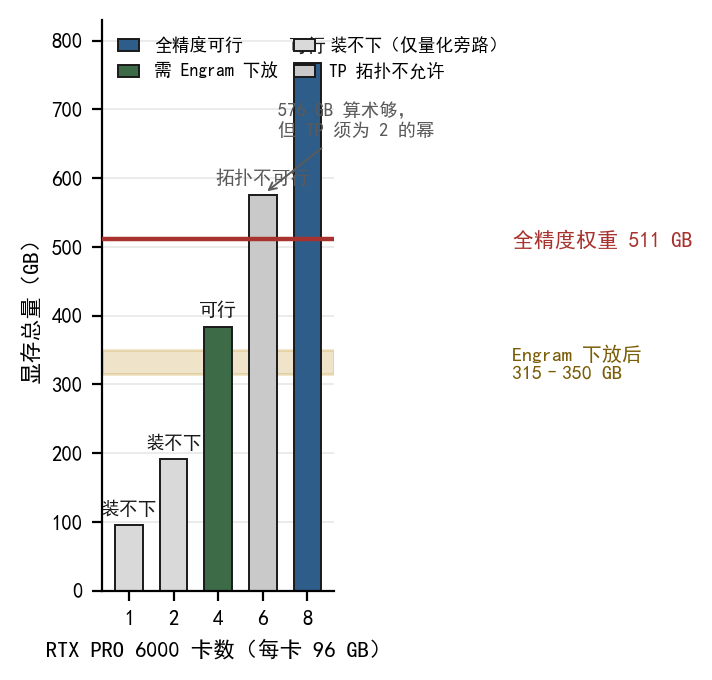
\includegraphics[width=0.86\textwidth]{../figures/fig-1.png}
\caption{装下 V4.1-Flash 需要几张 96 GB 卡。6 卡是本文最容易被忽略的一档：576 GB 算术够，但 TP 拓扑不允许。}
\label{fig:1}
\end{figure*}

\textbf{6 卡这一档值得单独说}：它算术上完全够（576 > 511），但任何主流框架都不会用它做 TP；只能用 TP2×PP3 这类流水并行，而那会引入气泡并让长上下文更难。\textbf{「算术够」与「拓扑允许」是两件事}，这是容量规划里最容易漏的一步。


\subsection{4 卡为什么能行}

511 GB 里有 196B 是 Engram，其 FP8 表在 TP 组内分片后实测占 \textbf{188.83 GiB}。 {\scriptsize\texttt{[c-\hspace{0pt}engram-\hspace{0pt}188gib]}}把它整体搬到主机内存（\texttt{--engram-config '\{"placement":"cpu"\}'}），腾出的 HBM 就够放剩余权重与 KV。代价是主机 RAM 与更长的加载时间。


第三方给出的「全部驻留」测算是约 614 GB，而 Engram 下放后仍需约 \textbf{315-\hspace{0pt}350 GB} 权重驻留显存。4 × 96 = 384 GB 恰好落在这个区间之上——\textbf{余量约 34-\hspace{0pt}69 GB，够 KV、激活与通信缓冲}。 {\scriptsize\texttt{[c-\hspace{0pt}min-\hspace{0pt}4x96]}}这就是 4 卡可行的算术依据。


\subsection{显存实际被谁吃掉了}

vLLM 路线在 8 卡上的实测很说明问题：\textbf{每卡约 91 GB / 96 GB}，而作者明确指出「Engram 表占主导：两张约 100 GB 的分片，整个 TP 组合计 189 GiB」。 {\scriptsize\texttt{[c-\hspace{0pt}tp8-\hspace{0pt}on-\hspace{0pt}8x96]}}换句话说，\textbf{吃掉显存的是 Engram，不是 KV}。


这与第 2.3 节完全一致：1M 上下文的 KV 只有 0.87 GiB，而 Engram 是 189 GiB——差两个数量级。



\section{硬件：Server Edition 特殊在哪}

\subsection{规格}

\begin{table*}[t]
\centering
\footnotesize
\setlength{\tabcolsep}{4pt}
\caption{RTX PRO 6000 三档变体的关键差异。}
\label{tab:4}
\begin{tabularx}{\textwidth}{llllX}
\toprule
项 & Server Edition & Workstation Edition & 备注 &  \\
\midrule
显存 & 96 GB GDDR7 & 96 GB GDDR7 & 三档相同 &  \\
带宽 & \textbf{1597 GB/s} & \textbf{1792 GB/s} & SE 低约 11\% & {\scriptsize\texttt{[c-\hspace{0pt}se-\hspace{0pt}spec]}} {\scriptsize\texttt{[c-\hspace{0pt}se-\hspace{0pt}vs-\hspace{0pt}ws-\hspace{0pt}bandwidth]}} \\
CUDA 核心 & 24,064 & 同 & 核心数相同 &  \\
FP4 / FP8 & 4 / 2 PFLOPS & 同 & 第五代 Tensor Core &  \\
最大功耗 & 600 W & 600 W & Max-Q 为 300 W &  \\
形态 & 被动散热 & 双槽吹风 & SE 需机箱风道 &  \\
显存超频 & \textbf{不支持} & 支持 & SE 返回错误 &  \\
\bottomrule
\end{tabularx}
\end{table*}

\subsection{三项差异，各自影响什么}

\textbf{（一）带宽低约 11\%。} 1597 / 1792 = 0.891（\textbf{推算}）。解码是带宽受限的（每生成一个 token 要把权重扫一遍），故 SE 的解码吞吐\textbf{按理论应比 WS 低约 11\%}。这是本文唯一一条关于「SE 比别的变体慢多少」的量化说法，且它\textbf{不是实测}。 {\scriptsize\texttt{[c-\hspace{0pt}se-\hspace{0pt}vs-\hspace{0pt}ws-\hspace{0pt}bandwidth]}}


\textbf{（二）没有显存超频。} 社区硬件页记录得很具体：Max-Q 卡接受显存时钟偏移，Server Edition 卡返回错误。而社区那组 4 卡数据（C1 249.1 tok/s）的条件恰是「Max-Q、325 W 功耗上限、显存 +6000」。故那组数字\textbf{双重不可迁移}：既是 MQ，又超了频。 {\scriptsize\texttt{[c-\hspace{0pt}r6k-\hspace{0pt}not-\hspace{0pt}se]}}


\textbf{（三）功耗不是瓶颈。} 这一条反直觉但证据一致：


\begin{itemize}
  \item 功耗扫描：600 W \sym{→}{} 500 W 几乎无差别；600 W \sym{→}{} 300 W 单用户仅损失约 4\%； {\scriptsize\texttt{[c-\hspace{0pt}power-\hspace{0pt}scaling]}}
  \item 现场实测：8 卡跑 128K 预填时 GPU 利用率约 87\%，但只吃到 \textbf{220 W / 600 W}。 {\scriptsize\texttt{[c-\hspace{0pt}prefill-\hspace{0pt}sgl-\hspace{0pt}8x]}}
\end{itemize}

两个独立来源指向同一结论：\textbf{这张卡在单流推理上根本吃不满 600 W}，瓶颈在别处（PCIe 通信、内核启动开销）。所以「SE 是 600 W 而 Max-Q 是 300 W」这个差别，在单流场景下\textbf{不构成性能差异}。


\subsection{被动散热的运维含义}

SE 是为服务器风道设计的（被动、单槽或液冷）。这意味着它\textbf{不能}像 WS 版那样塞进工作站机箱靠自身风扇散热。对本主题的实际影响是：多卡 SE 节点必然是机架式、有强风道。代价不在性能，在整机形态、噪音与供电。



\section{软件：为什么必须自带魔改镜像}

\subsection{上游 vLLM 在 SM120 上起不来}

这不是「性能差一点」，是\textbf{起不来}。社区做过逐条对账，列出四个独立阻塞点：


\begin{enumerate}
  \item \textbf{捆绑的 DeepGEMM 无 SM120 支持} —— FP8 权重处理时在 \texttt{layout.hpp:59} 断言失败
\end{enumerate}
   （\texttt{Unknown\allowbreak{} SF\allowbreak{} transformation}）；

\begin{enumerate}
  \item 设 \texttt{VLLM\_USE\_DEEP\_GEMM=0} 回退，则撞上 \textbf{CUTLASS c3x \texttt{dispatch\_scaled\_mm} RuntimeError} ——
\end{enumerate}
   上游同样没有 SM120 的 fp8-blockwise scaled-mm 内核；

\begin{enumerate}
  \item \texttt{VLLM\_TEST\_FORCE\_FP8\_MARLIN=1} 也无法绕开；
  \item 原文结论：「纯上游 vLLM 今天在 SM120 上无法服务 DeepSeek-V4-Flash（带不带 DSpark 都一样）」。 {\scriptsize\texttt{[c-\hspace{0pt}upstream-\hspace{0pt}vllm-\hspace{0pt}blocked]}}
\end{enumerate}

\textbf{这是硬件缺陷还是软件滞后？} 社区对 SM120 的技术澄清给出判断：SM120 缺的是 2-CTA 与 TMEM，但这两项「是为巨大 HBM 阵列与大规模扩展设计的，SM120 不需要它们就能打满算力与带宽」。真正的瓶颈是「软件分叉」——主流实验室的 kernel 开发优先服务 SM100 生产环境。 {\scriptsize\texttt{[c-\hspace{0pt}sglang-\hspace{0pt}no-\hspace{0pt}sm120]}}


\subsection{官方文档矩阵里没有 SM120}

SGLang 官方 cookbook 的每个 NVIDIA 单元格都用 preview 镜像，平台只有 H200 / B200 / B300 / GB300。SM120 \textbf{不在矩阵内}——不是「不推荐」，是「没有验证过的 recipe」。官方还明说该模型\textbf{尚未进入任何 SGLang release}，stock \texttt{pip\allowbreak{} install\allowbreak{} sglang} 无法服务它。 {\scriptsize\texttt{[c-\hspace{0pt}sglang-\hspace{0pt}no-\hspace{0pt}sm120]}}


第三方配置库是同一图景：Artificial Analysis 收录的 133 个配置里有 22 个是 V4.1-Flash，加速器清一色是数据中心卡（Vera Rubin NVL72 等），\textbf{无一例 RTX PRO 6000}。 {\scriptsize\texttt{[c-\hspace{0pt}aa-\hspace{0pt}no-\hspace{0pt}sm120]}}


\subsection{可用的三条路}

\begin{table*}[t]
\centering
\footnotesize
\setlength{\tabcolsep}{4pt}
\caption{在 SM120 上可用的栈与它们的代价。}
\label{tab:5}
\begin{tabularx}{\textwidth}{lXl}
\toprule
栈 & 镜像 & 状态 \\
\midrule
SGLang & \texttt{lmsysorg/sglang:dev-\allowbreak{}dsv41}（preview） & 官方文档指定；非 release \\
vLLM & \texttt{deepseekv41-\allowbreak{}flash-\allowbreak{}0909} 一类分支 & 现场报告自建 \\
社区整合 & 带 SM120 补丁的 DeepGEMM fork & 可用，但数字难归因 \\
\bottomrule
\end{tabularx}
\end{table*}

\textbf{一个必须接受的现实}：多数现场报告的镜像 commit 是 \texttt{unknown}、\texttt{pip\allowbreak{} show\allowbreak{} sglang} 是 \texttt{0.0.0.dev0}。这意味着\textbf{结果无法归因到任何特定 release}——你能复现的是「某台机器上的某个 build」，不是「SGLang 0.x.y」。这对生产选型是实质风险。 {\scriptsize\texttt{[c-\hspace{0pt}need-\hspace{0pt}forked-\hspace{0pt}image]}}


\subsection{几个会静默出错的配置点}

\textbf{（一）不要在 SGLang 里覆盖 backend。} 官方写明 \texttt{-\allowbreak{}-\allowbreak{}attention-\allowbreak{}backend}、\texttt{-\allowbreak{}-\allowbreak{}moe-\allowbreak{}runner-\allowbreak{}backend}、\texttt{-\allowbreak{}-\allowbreak{}fp8-\allowbreak{}gemm-\allowbreak{}backend} 由模型/硬件/前向模式/形状自动解析。覆盖它们是「最常导致失望测量结果的原因」——会把 32 宽的 ue8m0 块打到 Triton 回退上，吃掉大部分 bs=1 吞吐。


\textbf{（二）DSpark 是两个栈里唯一的投机路径。} 官方明确：\textbf{没有 EAGLE，也没有 MTP}，\texttt{-\allowbreak{}-\allowbreak{}speculative-\allowbreak{}num-\allowbreak{}steps} 这个旋钮不存在（草稿 token 数从 checkpoint 解析）。


\textbf{（三）高吞吐配方会关掉投机。} 官方解释：DSpark 一步的成本显著高于普通解码步，故 bs=1 的收益约等于「接受长度 ÷ 该固定步成本」；大批量时固定成本收不回来。这条和现场实测完全一致（见第 6.3 节）。


\textbf{（四）PD 分离在非 SM100 上要显式改 backend。} 两个角色默认都跑 MegaAttention，但那只在 SM100/SM103 上；解码端若在别的 GPU 上，预填端也必须设 \texttt{-\allowbreak{}-\allowbreak{}dsv4-\allowbreak{}attn-\allowbreak{}backend\allowbreak{} flashmla}，否则首个请求就以 \texttt{KV\allowbreak{} layout\allowbreak{} mismatch} 失败。



\section{实测：SE 只有一格，其余来自 Max-Q 或未标变体}

\subsection{Server Edition 上究竟测过什么}

先把这一格说清楚，因为它是本文的起点。把社区记录按「卡数 × 变体 × 是否限功耗」排开，\textbf{只有一格有完整吞吐}：


\begin{table*}[t]
\centering
\footnotesize
\setlength{\tabcolsep}{4pt}
\label{tab:6}
\begin{tabularx}{\textwidth}{lllXlll}
\toprule
配置 & 变体 & 功耗 & 单流解码 & 16/8 流聚合 & 预填 & 出处 \\
\midrule
4 卡 + Engram 放 RAM & \textbf{Server Edition} & 450 W（限功耗） & 183 tok/s & 695 tok/s（16 流） & 18,400-\hspace{0pt}19,200 tok/s & {\scriptsize\texttt{[c-\hspace{0pt}se-\hspace{0pt}measured-\hspace{0pt}but-\hspace{0pt}thin]}} \\
\textbf{8 卡（TP4+EP4 单副本）} & \textbf{Server Edition} & 默认 & 403.5（code） & 4,404 @ C=128 & — & {\scriptsize\texttt{[c-\hspace{0pt}se-\hspace{0pt}8x-\hspace{0pt}measured]}} \\
2 卡（剪枝 224/384） & 未标注 & 默认 & 141 & 288（3 流） & \textasciitilde{}9,800 & {\scriptsize\texttt{[c-\hspace{0pt}prune-\hspace{0pt}route]}} \\
8 卡 & Max-Q & 325 W + 显存超频 & 36.5-\hspace{0pt}252 tok/s & — & 6,853 tok/s & {\scriptsize\texttt{[c-\hspace{0pt}prefill-\hspace{0pt}sgl-\hspace{0pt}8x]}} \\
4 卡 & Max-Q & 默认 & 115.2-\hspace{0pt}249.1 tok/s & 468.2-\hspace{0pt}805.5 tok/s & 17,982 tok/s & {\scriptsize\texttt{[c-\hspace{0pt}decode-\hspace{0pt}tp4-\hspace{0pt}conc]}} \\
2 卡 + EXL3 3-bit & Max-Q & 350 W & 163.6-\hspace{0pt}202.9 tok/s（实测多用 200-\hspace{0pt}300） & 361.6 tok/s（4 流） & 约 11.9k tok/s & {\scriptsize\texttt{[c-\hspace{0pt}exl3-\hspace{0pt}2x-\hspace{0pt}throughput]}} \\
\bottomrule
\end{tabularx}
\end{table*}

三个必须同时说的事实：


\textbf{（一）那唯一一格不是默认配置。} 4×SE 那组把 Engram 表放在主机 RAM、并把功耗限到 450 W（默认 600 W）。所以它回答的是「SE 在省电且牺牲显存余量时能跑多快」，不是「SE 出厂默认能跑多快」。这两者不能互相代入。


\textbf{（一·补）两条 SE 与 Max-Q 的硬性差异。} 这两条不是调优偏好，是设备直接拒绝：


\begin{itemize}
  \item \textbf{显存超频。} Max-Q 接受显存时钟偏移（社区常用 +4000，换来「几个百分点」），
\end{itemize}
  \textbf{Server Edition 设置该偏移会返回错误}。 {\scriptsize\texttt{[c-\hspace{0pt}se-\hspace{0pt}no-\hspace{0pt}mem-\hspace{0pt}overclock]}}  故任何在 Max-Q 上靠超频跨过的性能门槛，在 SE 上按原样配置会差一点点，  且不会报错——只会慢。

\begin{itemize}
  \item \textbf{RAM Engram 的代价是硬性的。} 按 TP4 历史账目，表本身 188.83 GiB，
\end{itemize}
  另加 loader / server / OS 内存；且 \textbf{RAM 分配失败不会静默退回磁盘模式}。 {\scriptsize\texttt{[c-\hspace{0pt}engram-\hspace{0pt}ram-\hspace{0pt}need]}}  也就是说「内存不够就自动降级」是错的，实际是启动失败。


\textbf{（二）8 卡 SE 也有吞吐，但拓扑是「两个 4 卡副本」。} 同一台 8×SE 节点（云 VM、EPYC 9B45、1.4 TB RAM）用同一镜像跑 8 卡，\textbf{一次只跑一个 TP4+EP4 副本}：单流 code 403.5 tok/s（峰值 484）、codegen 444.6，codeconc 聚合 C=1/8/32/64/128 为394 / 1,301 / 2,509 / 3,439 / \textbf{4,404 tok/s}，128 流长生成 2,634。 {\scriptsize\texttt{[c-\hspace{0pt}se-\hspace{0pt}8x-\hspace{0pt}measured]}}互连另有实测：NCCL 总线带宽 37.6 GB/s（默认仅 22.2，需 \texttt{NCCL\_MIN\_NCHANNELS=8}）。 {\scriptsize\texttt{[c-\hspace{0pt}se-\hspace{0pt}measured-\hspace{0pt}but-\hspace{0pt}thin]}}\textbf{故仍空白的不是「8 卡 SE」，而是「8 卡当单个 TP8 副本用」。}这两者是不同的配置：同一台机器上，把 8 卡切成两个 TP4 副本可以并发两个请求流，而做成一个 TP8 副本要在 PCIe 无 NVLink 上跨 8 卡 all-reduce，代价无人公开测过。同页 released head（k=3）的对照值为 4,658 tok/s @ C=128，{\scriptsize\texttt{[c-\hspace{0pt}se-\hspace{0pt}8x-\hspace{0pt}measured]}}可见 tuned head 的增益在 C=128 上反而被摊薄——投机解码在高并发下帮不上忙。


\textbf{（三）卡多不等于快——这条反直觉，但被两组数据同时支持。}4×SE 的预填 18,400-\hspace{0pt}19,200 tok/s 是 8×Max-Q 的 6,853 tok/s 的 \textbf{2.7-\hspace{0pt}2.8 倍}。 {\scriptsize\texttt{[c-\hspace{0pt}se-\hspace{0pt}measured-\hspace{0pt}but-\hspace{0pt}thin]}}卡更少、变体更慢（1597 vs 1792 GB/s）、功耗更低，预填反而快得多。原因不在算力而在拓扑：8 卡走 PCIe、无 NVLink 时，张量并行的 all-reduce 把预填拖成通信受限（实测只吃到 600 W 中的 220 W）。 {\scriptsize\texttt{[c-\hspace{0pt}prefill-\hspace{0pt}ceiling]}}\textbf{所以「这个模型要几张卡」与「这个模型在哪台机器上更快」是两个问题。}


于是本文的写法是：机制层面（显存算术、TP 约束、软件栈、失败模式）给出结论，并说明它们在 SE 上如何变化；吞吐层面只报「哪台机器、什么配置、多少」，不做跨机器的「约等于」。


\subsection{先把边界钉死}

\begin{table*}[t]
\centering
\footnotesize
\setlength{\tabcolsep}{4pt}
\label{tab:7}
\begin{tabularx}{\textwidth}{lXl}
\toprule
来源 & 硬件原话 & 变体 \\
\midrule
vLLM 现场报告 & 「8x RTX PRO 6000 96GB」 & \textbf{未标明} \\
SGLang 现场报告 & 「8× RTX PRO 6000 Blackwell Max-Q」 & Max-Q \\
社区 4 卡 & 「Max-Q、325 W、显存 +6000」 & Max-Q（超频） \\
EXL3 量化 & 「two RTX PRO 6000 Blackwell Max-Q」 & Max-Q \\
\bottomrule
\end{tabularx}
\end{table*}

\textbf{故：本文所有吞吐数字都是 MQ 或未标变体的，SE 上一个都没有。} {\scriptsize\texttt{[c-\hspace{0pt}se-\hspace{0pt}measured-\hspace{0pt}but-\hspace{0pt}thin]}}


可迁移的部分：显存算术（96 GB 三档相同）、TP 约束、软件栈、失败模式、「功耗不是瓶颈」的结论（SE 更是 600 W，只会更不吃紧）。


不可迁移的部分：任何绝对吞吐数字。按带宽比推算，SE 的\textbf{解码}吞吐约低 11\%；预填受算力而非带宽限制，且实测吃不满功耗，故预填的差别应小于 11\%——但这是推算。


\subsection{预填：约 7K tok/s 是无 NVLink 的天花板}

SGLang，8 卡 PCIe（\textbf{无 NVLink}），128K 冷预填：


\begin{table*}[t]
\centering
\footnotesize
\setlength{\tabcolsep}{4pt}
\caption{128K 冷预填的配置扫描：前四行落在噪声内，后两行是真回退。}
\label{tab:8}
\begin{tabularx}{\textwidth}{Xll}
\toprule
配置 & tok/s &  \\
\midrule
\texttt{chunked\_prefill\_size=2048}（生产） & \textbf{6,853} & {\scriptsize\texttt{[c-\hspace{0pt}prefill-\hspace{0pt}sgl-\hspace{0pt}8x]}} \\
同配置重跑 & 6,765（−1.3\%） &  \\
\texttt{flashmla} 预填后端 & 6,845 &  \\
fused-MoE all-reduce & 6,828 &  \\
\texttt{chunked\_prefill\_size=4096} & 6,301 &  \\
\texttt{chunked\_prefill\_size=1024} & 6,012 &  \\
\bottomrule
\end{tabularx}
\end{table*}

\textbf{怎么读这张表}：作者自己后来更正——\texttt{flashmla}（6,845）与 fused-MoE（6,828）都落在生产重跑（6,853 对 6,765）的 ±1.3\% 内，正确读法是「\textbf{无可检测差异}」，不是「这两个变体更慢」。单次重跑不是噪声估计，1.3\% 的差不能用来排名。


真正的信号是资源占用：32K 提示约 7,196 tok/s，\textbf{GPU 利用率约 87\% 但只吃到 220 W / 600 W}。作者据此判断「瓶颈是 PCIe 通信，不是算力」，并给出「这块板子无 NVLink 时约 7K tok/s 是天花板」。


\textbf{最可迁移的一条}：4 卡档实测 4,714 token 冷提示 0.788 s ≈ 5,982 tok/s——卡数减半，预填只降 13\%，进一步证明不是算力受限。


\textbf{唯一的大倍率来自前缀缓存}：112K token 前缀命中时 0.34 s ≈ \textbf{325K tok/s（约 39 倍）}。 {\scriptsize\texttt{[c-\hspace{0pt}prefill-\hspace{0pt}ceiling]}}


\subsection{解码：投机解码是「可用 vs 不可用」}

SGLang，8 卡，单流：


\begin{table*}[t]
\centering
\footnotesize
\setlength{\tabcolsep}{4pt}
\caption{DSpark 开关的 A/B：关掉后无论提示类型都塌到约 36.5 tok/s。}
\label{tab:9}
\begin{tabular}{lll}
\toprule
提示类型 & DSpark 开 & DSpark 关 \\
\midrule
散文 & 76.5-\hspace{0pt}78.9 tok/s & 36.4-\hspace{0pt}36.5 tok/s \\
结构化 / JSON & 120.3-\hspace{0pt}120.5 tok/s & 36.5 tok/s \\
接受长度 & 3.0 token/步 & 1.0 \\
\bottomrule
\end{tabular}
\end{table*}

\begin{figure*}[t]
\centering
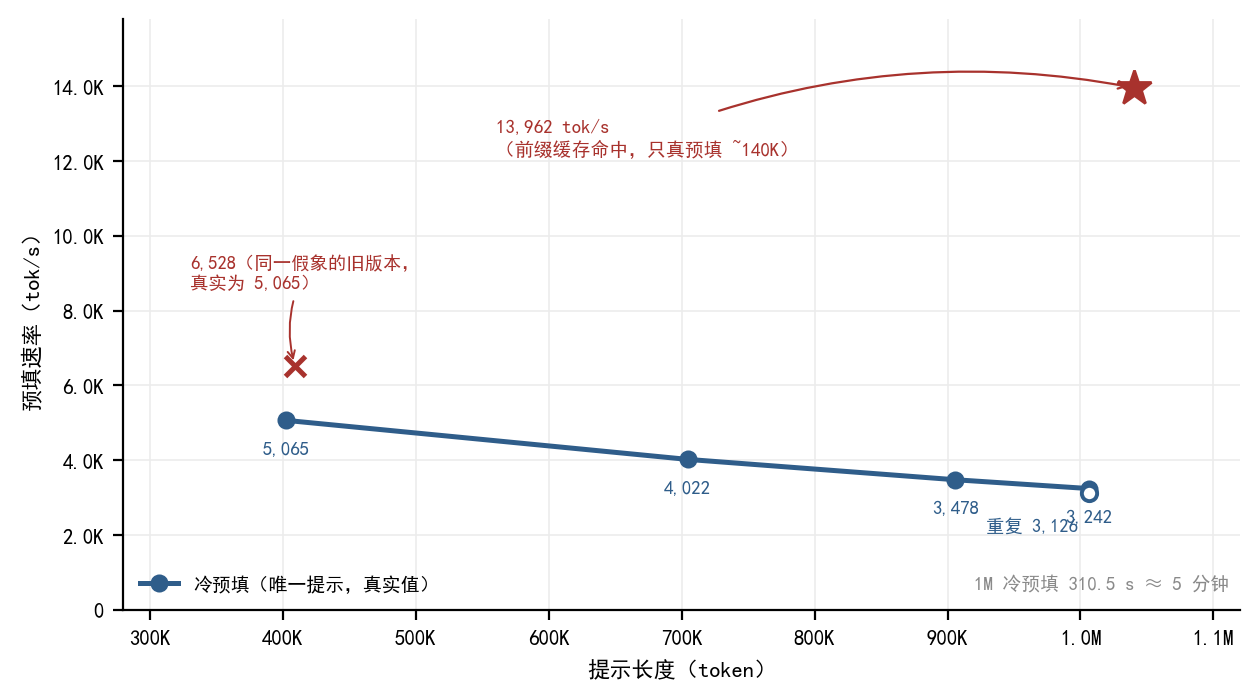
\includegraphics[width=0.86\textwidth]{../figures/fig-2.png}
\caption{预填速率随上下文衰减，以及两个高出 3-\hspace{0pt}4 倍的假象（前缀缓存命中）与真实冷值的对比。}
\label{fig:2}
\end{figure*}

\textbf{关掉投机后，模型无论提示类型都塌到约 36.5 tok/s。} 作者的判断是：「投机是这个硬件上『可用』与『不可用』延迟的分界」。生产用 \texttt{block\_size=6} 时结构化提示约 \textbf{237-\hspace{0pt}252 tok/s}。 {\scriptsize\texttt{[c-\hspace{0pt}decode-\hspace{0pt}dspark]}}


这与官方文档互相印证：DSpark 的接受率\textbf{强依赖负载}（数学/代码最高，开放聊天较低，agentic trace 更低），且一步的成本不随接受长度或草稿块大小变化——所以调 \texttt{block\_size} 不会买来吞吐，只会改变「在哪个负载上更划算」。


\subsection{并发：2 是免费的，8 是硬上限}

4 卡 TP4/EP4 的并发曲线：


\begin{table*}[t]
\centering
\footnotesize
\setlength{\tabcolsep}{4pt}
\caption{4 卡 TP4/EP4 的并发扩展：8 并发合计 4.06×，但每流速率已降到 66.2 tok/s。}
\label{tab:10}
\begin{tabular}{rrrrll}
\toprule
并发 & 合计 tok/s & 相对 1 & 每流 tok/s & TTFT & TPOT \\
\midrule
1 & 115.2 & 1.00× & 121.9 & 0.121 s & 8.2 ms \\
2 & 220.6 & 1.91× & 125.8 & 0.147 s & 8.0 ms \\
4 & 322.2 & 2.80× & 108.5 & 0.643 s & 9.3 ms \\
8 & 468.2 & 4.06× & 66.2 & 0.157 s & 15.2 ms \\
\bottomrule
\end{tabular}
\end{table*}

\begin{figure*}[t]
\centering
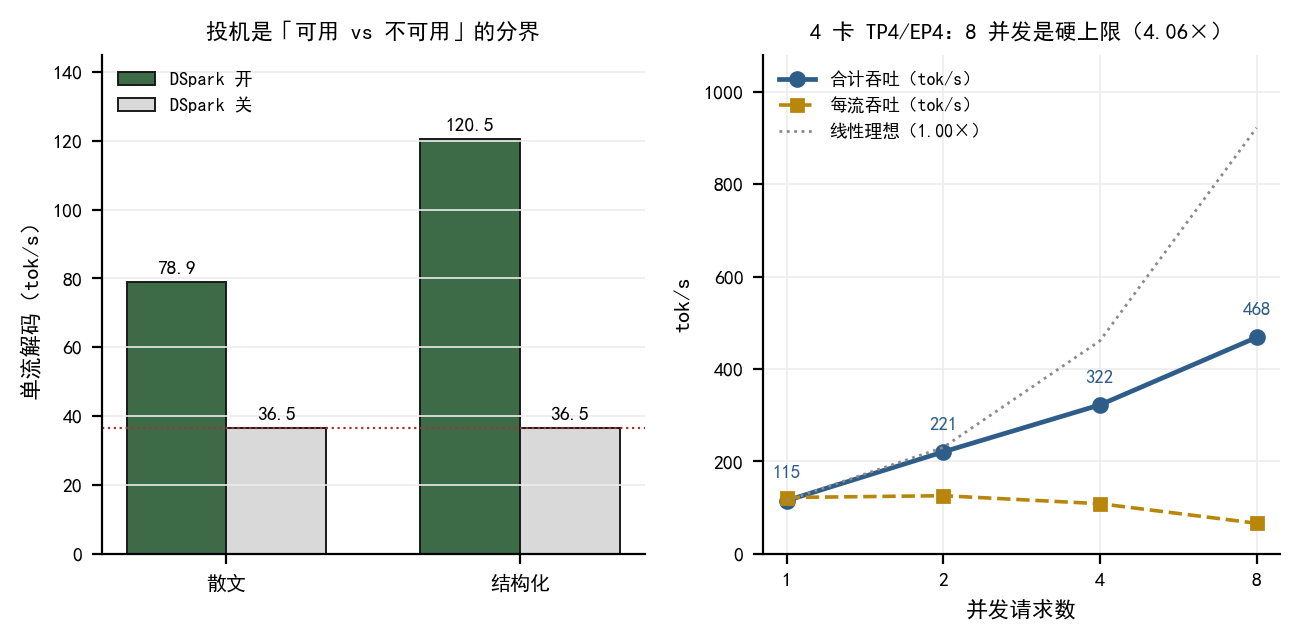
\includegraphics[width=0.86\textwidth]{../figures/fig-3.png}
\caption{解码侧的两件事：投机开关决定量级（左），并发最多 4 倍（右）。}
\label{fig:3}
\end{figure*}

\textbf{并发 2 是免费的}（每流速率不降反升），8 是硬上限（\texttt{max\_running\_requests=8} 且 decode 图只捕到 bs=8）。作者明说 N=2，\textbf{不是误差棒}，应读作首轮而非定表。 {\scriptsize\texttt{[c-\hspace{0pt}decode-\hspace{0pt}tp4-\hspace{0pt}conc]}}


社区 4 卡（MQ 325 W，超频）的另一组稳定配置：C1 \textbf{249.1 tok/s}、C8 合计 \textbf{805.5 tok/s}、32K 预填 \textbf{17,982 tok/s}、4,727,748 逻辑 KV token。 {\scriptsize\texttt{[c-\hspace{0pt}stable-\hspace{0pt}tp4-\hspace{0pt}profile]}}比上面那组高得多，差别在 adaptive DSpark K7 与更激进的调优。\textbf{两组不可直接比较}——硬件条件与镜像都不同。


\subsection{1M 上下文：能跑，但要 5 分钟}

SGLang，4 卡，冷预填阶梯（每行提示带唯一标记，保证不是缓存命中）：


\begin{table*}[t]
\centering
\footnotesize
\setlength{\tabcolsep}{4pt}
\caption{1M 冷预填阶梯：随上下文增长单调下降，全程约 5 分钟。}
\label{tab:11}
\begin{tabular}{lll}
\toprule
提示 token & 耗时 & 预填速率 \\
\midrule
402,625 & 79.5 s & 5,065 tok/s \\
704,582 & 175.2 s & 4,022 tok/s \\
905,885 & 260.5 s & 3,478 tok/s \\
1,006,538 & 310.5 s & \textbf{3,242 tok/s} \\
1,006,538（重复） & 322.0 s & 3,126 tok/s \\
\bottomrule
\end{tabular}
\end{table*}

\textbf{结论：一次完整的 1M 冷预填约 5 分钟。} {\scriptsize\texttt{[c-\hspace{0pt}1m-\hspace{0pt}cold-\hspace{0pt}5min]}}


\textbf{而流传的「1040K 在 74.5 秒内完成（13,962 tok/s）」是假象}：那 900K 前缀已在 radix cache 里，实际只预填了约 140K。作者不仅更正了这个数，还更正了自己更早的「409K = 62.7 s（6,528 tok/s）」——真实冷数字是 79.5 s（5,065 tok/s）。 {\scriptsize\texttt{[c-\hspace{0pt}cache-\hspace{0pt}artifact]}}


vLLM 路线独立验证了「1M 能跑」：950K token 双针检索正确，预填 4,584 tok/s（纯 torch logits、eager 模式）。\textbf{「能跑」与「跑得快」是两件事}：4,584 对 SGLang 的 6,853（上下文长度不同，不可直接比）。 {\scriptsize\texttt{[c-\hspace{0pt}vllm-\hspace{0pt}1m-\hspace{0pt}verified]}}


\subsection{长上下文的并发会塌}

同一 4 卡机，906K 上下文：


\begin{itemize}
  \item 单请求重复 5 次：解码 100 tok/s、TPOT 10 ms、TTFT 2.38 s（对比冷预填 260 s，前缀缓存值 \textbf{109 倍}）；
  \item \textbf{4 个并发}（各 906K 上下文、各 256 输出 token）：合计 8.6 s，\textbf{仅 29.7 tok/s}（每流约 7.4）。
\end{itemize}

作者的判断很直接：\texttt{max\_running\_requests=8} 在这个上下文规模下是名义值；\textbf{这个端点擅长服务一个重请求，而不是多个}。 {\scriptsize\texttt{[c-\hspace{0pt}long-\hspace{0pt}ctx-\hspace{0pt}collapse]}}


\subsection{显存天花板}

\begin{table*}[t]
\centering
\footnotesize
\setlength{\tabcolsep}{4pt}
\caption{两条独立路线撞到同一面墙：96 GB 是硬边界，余量约 1 GB。}
\label{tab:12}
\begin{tabular}{llll}
\toprule
路线 & 实测峰值 & 上限 & 余量 \\
\midrule
SGLang 4 卡 1M 配置 & 96.8 GB & 97.9 GB（98.9\%） & \textasciitilde{}1 GB \\
EXL3 2 卡 1.04M 提示 & 96,655 MiB & 97,887 MiB & \textasciitilde{}1.2 GB \\
EXL3 2 卡 1.04M 提示 & 97,029 MiB & 97,887 MiB & \textasciitilde{}0.8 GB \\
\bottomrule
\end{tabular}
\end{table*}

\textbf{两条独立路线撞到同一面墙。} 96 GB 是硬边界，且余量只有约 1 GB—— {\scriptsize\texttt{[c-\hspace{0pt}vram-\hspace{0pt}ceiling]}}「跑两个长请求」之前必须先算这笔账。



\section{失败模式：哪些报错，哪些静默}

这一节按「失败是否可见」排序，因为\textbf{静默的比报错的危险得多}。


\subsection{静默失败}

\begin{table*}[t]
\centering
\footnotesize
\setlength{\tabcolsep}{4pt}
\caption{五类失败模式，按「失败是否可见」排序。}
\label{tab:13}
\begin{tabularx}{\textwidth}{XllXX}
\toprule
坑 & 类型 & 触发条件 & 为什么危险 &  \\
\midrule
\textbf{FP8 KV 的 scale 布局} & 静默 & 短提示全过，≥100K 暴露 & {\scriptsize\texttt{[c-\hspace{0pt}fp8-\hspace{0pt}kv-\hspace{0pt}layout-\hspace{0pt}pitfall]}} 块布局是 `[64tok×128B fp8 \textbackslash{} & 64tok×4B fp32 scale]`（块尾追加），不是逐 token 交错。理解错就是\textbf{数值损坏}，不报错 \\
\textbf{前缀缓存假象} & 静默 & 共享前缀的提示 & {\scriptsize\texttt{[c-\hspace{0pt}cache-\hspace{0pt}artifact]}} radix cache 会保留已完成请求的页，虚高 3-\hspace{0pt}4 倍。作者自己的两组数都中招 &  \\
\textbf{\texttt{-\allowbreak{}-\allowbreak{}enable-\allowbreak{}dp-\allowbreak{}attention} 单独用} & 静默 & 单独启用 & \texttt{dp\_size} 仍是 1。会让人把\textbf{旧配置当成新配置}记录，整轮数据作废 & {\scriptsize\texttt{[c-\hspace{0pt}sgl-\hspace{0pt}rejects-\hspace{0pt}dp]}} \\
\textbf{容器没传 \texttt{-e TP\_SIZE}} & 静默 & 漏传环境变量 & 服务照常起，跑的是默认 TP8。作者记录「整轮假数据」就是这么来的 &  \\
\textbf{镜像未标 commit} & 静默 & 用社区 build & 数字无法归因到任何 release；\texttt{pip\allowbreak{} show\allowbreak{} sglang} 可能是 \texttt{0.0.0.dev0} &  \\
\bottomrule
\end{tabularx}
\end{table*}

\textbf{应对方法的来源里给了现成的}：用 \texttt{-\allowbreak{}-\allowbreak{}enable-\allowbreak{}cache-\allowbreak{}report}，每行断言\texttt{usage.prompt\_tokens\_details.cached\_tokens\allowbreak{} ≈\allowbreak{} 0}；用 \texttt{/get\_server\_info} 核对生效配置再计时。更细的一条是——SGLang 只在 \texttt{cached\_tokens\allowbreak{} >\allowbreak{} 0} 时才发 \texttt{prompt\_tokens\_details}，故冷行该字段\textbf{缺失而非 0}，harness 要按 \texttt{or \{\}} 默认为 0，否则最想要的冷行会被丢掉。


\subsection{会报错或挂死的}

\begin{table*}[t]
\centering
\footnotesize
\setlength{\tabcolsep}{4pt}
\label{tab:14}
\begin{tabularx}{\textwidth}{XXl}
\toprule
坑 & 表现 &  \\
\midrule
DeepGEMM autotune 挂死 & 首次长上下文批（128K+）deadlock，bring-up 需跳过或 eager & {\scriptsize\texttt{[c-\hspace{0pt}deepgemm-\hspace{0pt}hang]}} \\
FlashInfer sparse-MLA SM120 实例化缺口 & 部分 \texttt{(num\_heads,\allowbreak{} topk)} 组合（如 \texttt{(16, 512)}）不在分发表里，视觉路径同样中招 &  \\
CUDA graph 捕获崩溃 & flashinfer 算子在图里、>4K token 时崩；作者用纯 torch 替换后正常 &  \\
SGLang 拒绝 DP 拓扑 & DP2×TP4 抛「V4.1 vision currently supports TP/EP without DP, CP, PP or MoE A2A」，两副本约 70 s 内死亡 & {\scriptsize\texttt{[c-\hspace{0pt}sgl-\hspace{0pt}rejects-\hspace{0pt}dp]}} \\
整个 TP 组被 SIGKILL（Exited 137） & 未复现；最可疑原因是冷启动后首个超大请求触发 Triton 形状 JIT，卡过 300 s 看门狗 &  \\
\bottomrule
\end{tabularx}
\end{table*}

\textbf{一条运维规矩值得抄下来}：冷启动后先发一个几百 K token 的预热请求并等它完成，再信任服务。另外，\texttt{docker\allowbreak{} rm\allowbreak{} -\allowbreak{}f} 可能杀不掉 defunct 容器，而孤儿引擎进程仍占端口并应答健康检查——于是下一次实验会被静默标错。要循环 \texttt{docker\allowbreak{} rm\allowbreak{} -\allowbreak{}f} 直到端口真的没人监听。


\subsection{性能回退}

\textbf{MXFP4 专家路径在 SM120 上回退到 Marlin 内核}（上游已知 issue）。能跑，性能损失被作者评为「可接受」。这不是可以「修好」的配置问题，是内核覆盖缺口。 {\scriptsize\texttt{[c-\hspace{0pt}marlin-\hspace{0pt}fallback]}}



\section{自建还是 API}

\subsection{官方价目}

\begin{table*}[t]
\centering
\footnotesize
\setlength{\tabcolsep}{4pt}
\caption{官方 API 价目（deepseek-flash）。}
\label{tab:15}
\begin{tabular}{lll}
\toprule
项 & 值 &  \\
\midrule
输出 / 1M token（峰时） & \textbf{\$1.2} &  \\
输出 / 1M token（谷时） & \$0.6 &  \\
输入 / 1M token（缓存命中，峰时） & \textbf{\$0.006} &  \\
上下文 & 1M &  \\
并发上限 & \textbf{2,500} & {\scriptsize\texttt{[c-\hspace{0pt}api-\hspace{0pt}price]}} \\
\bottomrule
\end{tabular}
\end{table*}

谷时是峰时的 50\%，峰时为 UTC 周一至周五 01:00-\hspace{0pt}04:00 与 06:00-\hspace{0pt}10:00。


\subsection{量级对比（不是同条件对照）}

第三方给出的盈亏平衡点是：8×H200 节点（AWS 约 \$63/小时）要持续产出约 \textbf{14,650 输出 token/s}才能追平 \$1.2/百万 token。


本主题的实测：


\begin{table*}[t]
\centering
\footnotesize
\setlength{\tabcolsep}{4pt}
\caption{与盈亏平衡点的量级对比（跨硬件，仅作参照）。}
\label{tab:16}
\begin{tabular}{llll}
\toprule
场景 & 实测 & 与 14,650 的比 &  \\
\midrule
单流解码（4 卡，DSpark） & 115.2 tok/s & 1/127 &  \\
8 并发合计（4 卡） & 468.2 tok/s & 1/31 &  \\
8 并发合计（8 卡，社区调优） & 805.5 tok/s & 1/18 & {\scriptsize\texttt{[c-\hspace{0pt}selfhost-\hspace{0pt}breakeven]}} \\
\bottomrule
\end{tabular}
\end{table*}

\textbf{必须写明的限制}：14,650 那个数来自 \textbf{8×H200}，本文的实测来自 \textbf{4-\hspace{0pt}8×RTX PRO 6000}。两者不是同一台机器、不是同一价格、不是同一负载。故这个比值\textbf{只能作量级参照}，不能读成「自建贵 31 倍」。


即便如此，量级差是清楚的：\textbf{自建的理由是数据主权、可微调、提示不出 VPC，不是省钱。}MIT 许可让这些成为可能（可商用、可微调、可再分发）。 {\scriptsize\texttt{[c-\hspace{0pt}selfhost-\hspace{0pt}for-\hspace{0pt}control]}}


\subsection{另一条硬件路线的代价}

vLLM-Ascend 给出了在 8×128 GB NPU 上部署的完整配方，但代价具体：必须 W8A8 权重 + INT8 Engram，且必须显式 \texttt{VLLM\_USE\_V2\_MODEL\_RUNNER=0}。 {\scriptsize\texttt{[c-\hspace{0pt}ascend-\hspace{0pt}alt]}}列在这里是为了说明「换平台不是换个 kernel，是换一套精度方案」。



\section{三档部署方案}

\begin{table*}[t]
\centering
\footnotesize
\setlength{\tabcolsep}{4pt}
\caption{三档部署方案与各自的实测/质量代价。}
\label{tab:17}
\begin{tabularx}{\textwidth}{lllXXX}
\toprule
方案 & 卡数 & 精度 & 栈 & 关键实测 &  \\
\midrule
A & 8×96 GB & 全精度 & SGLang TP8/EP8 或 vLLM TP8 & 128K 预填 6,853 tok/s；1M 可跑 &  \\
B & 4×96 GB & 全精度 & SGLang TP4/EP4 + Engram 下放 & C1 115.2；C8 468.2；1M 冷预填 310.5 s &  \\
C & 2×96 GB & EXL3 3-bit & 量化旁路 & agentic 224.1 tok/s；40K 预填 11,157/11,467；KL 0.0522（噪声底 0.0082 的 6.4 倍） & {\scriptsize\texttt{[c-\hspace{0pt}exl3-\hspace{0pt}throughput]}} {\scriptsize\texttt{[c-\hspace{0pt}quant-\hspace{0pt}quality-\hspace{0pt}cost]}} \\
\bottomrule
\end{tabularx}
\end{table*}

\subsection{方案 A：8×96 GB，全精度}

\begin{itemize}
  \item 栈：SGLang \texttt{dev-dsv41} 镜像，TP8/EP8，\texttt{-\allowbreak{}-\allowbreak{}mem-\allowbreak{}fraction-\allowbreak{}static\allowbreak{} 0.72}，fp8\_e4m3 KV；
  \item 或 vLLM 分支，TP=8，\texttt{-\allowbreak{}-\allowbreak{}kv-\allowbreak{}cache-\allowbreak{}dtype\allowbreak{} fp8\allowbreak{} -\allowbreak{}-\allowbreak{}block-\allowbreak{}size\allowbreak{} 128\allowbreak{} -\allowbreak{}-\allowbreak{}gpu-\allowbreak{}memory-\allowbreak{}utilization\allowbreak{} 0.85}；
  \item 实测：128K 冷预填约 6.8K tok/s、1M 上下文可跑、单流约 115-\hspace{0pt}249 tok/s（视调优）；
  \item 前提：接受魔改镜像；Engram 放主机内存或分片显存。
\end{itemize}

\subsection{方案 B：4×96 GB，全精度}

\begin{itemize}
  \item 栈：SGLang TP4/EP4，\texttt{--engram-config '\{"placement":"cpu"\}'}；
  \item 实测：C1 115.2 tok/s、8 并发 468.2 tok/s、1M 冷预填约 5 分钟、峰值 VRAM 98.9\%；
  \item 前提：主机 RAM 要够放 188.83 GiB 的 Engram 表；镜像必须自带 SM120 补丁。
\end{itemize}

\subsection{方案 C：2×96 GB，EXL3 3-bit}

\begin{itemize}
  \item 实测：\textbf{agentic 单会话解码 224.1 tok/s}（同轮墙钟 228.7 s）；固定提示下 2K 单流 156.9、
\end{itemize}
  \textbf{46K 单流中位 172.8}、46K 四流聚合 362.9；\textbf{40K 冷预填 11,157 / 11,467 tok/s}。 {\scriptsize\texttt{[c-\hspace{0pt}exl3-\hspace{0pt}throughput]}}

\begin{itemize}
  \item 质量代价是\textbf{可量化的，且不在噪声内}：原模型自身重跑的 KL 噪声底为 \textbf{0.0082}（中性文本），
\end{itemize}
  而该包实测 \textbf{0.0522 / 0.0306 / 0.0111 / 0.0338}（中性 / 代码 / agentic / short100）——  中性文本上是噪声底的 \textbf{6.4 倍}。任务准确率则几乎不动：GSM8K-200 98.5\%\sym{→}{}99.0\%、  HumanEval 95.7\%\sym{→}{}97.6\%，这部分在噪声内。 {\scriptsize\texttt{[c-\hspace{0pt}quant-\hspace{0pt}quality-\hspace{0pt}cost]}}

\begin{itemize}
  \item 故这条旁路的代价是三条：KL 偏离可测（6.4×）、引入非上游量化内核与打包格式、
\end{itemize}
  以及依赖主机 RAM（Engram int4 111 GB 常驻 pinned RAM）与磁盘。 {\scriptsize\texttt{[c-\hspace{0pt}exl3-\hspace{0pt}throughput]}}


\subsection{不推荐的做法}

\begin{itemize}
  \item \textbf{按 16B 估显存}：会得出「一张卡够」的错误结论，差 44 倍；
  \item \textbf{直接用上游 vLLM/SGLang}：SM120 上起不来；
  \item \textbf{在 SGLang 里手动指定 backend}：会把 ue8m0 块打到 Triton 回退，吃掉大部分 bs=1 吞吐；
  \item \textbf{关掉投机解码}：解码塌到 36.5 tok/s；
  \item \textbf{用共享前缀的提示做吞吐基准}：会测出 39 倍虚高。
\end{itemize}


\section{讨论：三条判断与一条边界}

\subsection{判断一：能装，但要 4 张起}

552B+196B、约 511 GB 权重，96 GB 卡的下限是 4 张（Engram 下放主机内存），2 张只能靠 3-bit 量化。TP 必须是 2 的幂，故 6 张这种「算术够、拓扑不行」的配置不存在。


\subsection{判断二：瓶颈在软件与互连，不在带宽与功耗}

三条独立证据：GPU 只吃 220 W / 600 W；600 W\sym{→}{}300 W 单用户仅损约 4\%；4 卡预填只比 8 卡低 13\%。真正的限制是 PCIe（无 NVLink 时预填约 7K tok/s 封顶）与 SM120 的内核覆盖缺口。 {\scriptsize\texttt{[c-\hspace{0pt}prefill-\hspace{0pt}ceiling]}} {\scriptsize\texttt{[c-\hspace{0pt}upstream-\hspace{0pt}vllm-\hspace{0pt}blocked]}}


\subsection{判断三：测量纪律比调优更重要}

本主题里最大的数字错误不是配置写错，而是\textbf{把缓存命中当成冷预填}。13,962 tok/s 与 3,242 tok/s 差 4.3 倍，而两者跑的是同一个模型、同一台机器、同一个镜像。 {\scriptsize\texttt{[c-\hspace{0pt}cache-\hspace{0pt}artifact]}}同类问题还有：用 SSE chunk 数代替 \texttt{usage.completion\_tokens}（DSpark 打包 2-\hspace{0pt}5 token/chunk，会 3-\hspace{0pt}5 倍低报）、在有交互流量时做基准（20-\hspace{0pt}47\% 失真）、以及孤儿进程应答健康检查。


\subsection{边界：SE 的问题公开证据还不能回答}

全部实测来自 Max-Q 或未标变体的卡。按带宽比推算 SE 的解码应低约 11\%，预填差别应更小——但这是\textbf{推算}。 {\scriptsize\texttt{[c-\hspace{0pt}se-\hspace{0pt}vs-\hspace{0pt}ws-\hspace{0pt}bandwidth]}}要真正回答标题里的问题，需要有人在一台多卡 SE 的机器上重跑第 6 节的那几张表。


在那之前，本文的价值是：\textbf{把可迁移的部分与不可迁移的部分分开写清楚}，而不是给一个看起来精确的平均数。



\section{附录 A　证据等级与本文的取值}

\begin{table*}[t]
\centering
\footnotesize
\setlength{\tabcolsep}{4pt}
\label{tab:18}
\begin{tabular}{lll}
\toprule
等级 & 本文中的含义 & 本主题的实际情况 \\
\midrule
复现级 & 第二方在同机同配置重跑得到一致结果 & \textbf{0 条} \\
测量级 & 有人在其机器上实测并公布了配置 & 全部吞吐数字 \\
规格级 & 厂商公布，未经该负载验证 & 显存、带宽、TDP、参数 \\
推算级 & 由规格或实测推导，无直接观测 & SE 相对 WS/MQ 的偏差、容量边界 \\
\bottomrule
\end{tabular}
\end{table*}

\textbf{没有复现级证据这件事本身值得写在摘要里}：这个模型发布不到两个月，SM120 又不是官方支持的平台，所有数字都还停在「一家之言」的阶段。


本归档的 102 条引文\textbf{全部由脚本按锚点子串从快照里切出}，没有一条是手写的。第一次生成时产出 14 条过短引文（如「6,853」）——它们是原文子串、校验会通过，但对论证零贡献，于是加了最小长度 160 字符重生成。最终 E1 校验 102/102 通过、0 条无法校验。


\section{附录 B　主张清单（42 条）}

\begin{table*}[t]
\centering
\footnotesize
\setlength{\tabcolsep}{4pt}
\label{tab:19}
\begin{tabularx}{\textwidth}{llX}
\toprule
claim\_id & 置信 & 一句话 \\
\midrule
c-v41-is-552b-moe & high & 552B 骨干 + 196B Engram，8B/16B 激活 \\
c-active-not-total & high & 显存看总参数，算力看激活参数，差一个数量级 \\
c-kv-890-bytes & high & 全局 KV 890 B/token，为 V4-Flash 的 1/4 \\
c-kv-implication & high & 1M 上下文 KV 仅约 0.87 GiB \\
c-se-spec & high & SE：96 GB / 1597 GB/s / 600 W / 被动 \\
c-se-vs-ws-bandwidth & high & SE 带宽为 WS 的 89\%（推算） \\
c-no-1m-on-2x96 & medium & 2 卡装不下 511 GB \\
c-min-4x96 & medium & 4 卡是最低全精度配置 \\
c-tp8-on-8x96 & high & vLLM TP8 跑通，91/96 GB \\
c-engram-dominates & high & Engram 是最大单块权重，可下放主机内存 \\
c-sglang-no-sm120 & high & SGLang 官方矩阵不含 SM120 \\
c-aa-no-sm120 & medium & 第三方配置库无一例 RTX PRO 6000 \\
c-upstream-vllm-blocked & high & 上游 vLLM 在 SM120 上起不来 \\
c-need-forked-image & high & 必须自带魔改镜像 \\
c-prefill-sgl-8x & high & 128K 预填 6,853 tok/s，220 W \\
c-prefill-ceiling & high & 无 NVLink 约 7K 封顶；缓存 39 倍 \\
c-decode-dspark & high & 投机关掉塌到 36.5 tok/s \\
c-decode-tp4-conc & high & 4 卡分并发：C1 115.2、C8 468.2 \\
c-1m-cold-5min & high & 1M 冷预填 310.5 s，约 5 分钟 \\
c-cache-artifact & high & 13,962 tok/s 是缓存假象 \\
c-long-ctx-collapse & high & 4×906K 并发仅 29.7 tok/s \\
c-vram-ceiling & high & 峰值 98.9\%，余量约 1 GB \\
c-sgl-rejects-dp & high & SGLang 拒绝 DP 拓扑 \\
c-vllm-1m-verified & high & vLLM 验证 1M 上下文 \\
c-fp8-kv-layout-pitfall & high & FP8 KV scale 布局是静默坑 \\
c-marlin-fallback & high & MXFP4 落到 Marlin \\
c-deepgemm-hang & high & 首次长批 autotune 挂死 \\
c-stable-tp4-profile & high & 社区 4 卡：C1 249.1、C8 805.5 \\
c-r6k-not-se & high & 那组数据双重不可迁移（MQ＋超频） \\
c-engram-188gib & high & Engram 主机内存 188.83 GiB \\
c-power-scaling & high & 600\sym{→}{}300 W 仅损约 4\% \\
c-tp-power-of-2 & high & TP 须为 2 的幂 \\
c-api-price & high & 输出 \$1.2/Mtok，并发 2500 \\
c-selfhost-breakeven & medium & 盈亏平衡 14,650 tok/s \\
c-selfhost-for-control & medium & 自建为控制权非省钱 \\
c-minimum-viable & high & 三档：8 卡 / 4 卡 / 2 卡量化 \\
c-quant-quality-cost & high & EXL3 的 KL 是噪声底 6.4 倍，准确率在噪声内 \\
c-exl3-throughput & high & EXL3 2 卡：agentic 224.1 tok/s；40K 预填 11,157 \\
c-se-8x-measured & high & \textbf{8×SE 全精度：C=128 聚合 4,404 tok/s} \\
c-prune-route & high & 剪枝 224/384 专家：2 卡 141 tok/s，GPQA 92.9\% \\
c-vision-native & high & 原生支持图像，API 侧仅 flash 支持 \\
c-no-chat-template & high & 不含 Jinja chat template \\
c-decode-flops-flat & high & 上下文 ×256，解码 FLOPs 仅 +1/4 \\
c-ascend-alt & high & Ascend 路线需 W8A8 + INT8 Engram \\
c-se-measured-but-thin & high & \textbf{SE 有实测但只覆盖 4 卡/450W 一格} \\
c-se-no-mem-overclock & high & SE 不支持显存超频（返回错误） \\
c-engram-ram-need & high & RAM Engram 188.83 GiB，失败不降级 \\
\bottomrule
\end{tabularx}
\end{table*}

\section{附录 C　复现路径与失败抓取}

\begin{lstlisting}
cd research/pro6000se-dsv41
python fetch.py ... fetch7.py    # 抓 20 份快照
python add_exl3_evidence.py      # 补 EXL3 的真实测量引文
python build_evidence.py         # 锚点扩窗生成 108 条引文（非手写）
python build_tables.py           # sources + claims，含引用闭合校验
python build_run.py              # run.json（轨迹 + 预算 + 缺口）
cd ../.. && python scripts/validate_research.py research/pro6000se-dsv41
python scripts/audit_paper.py research/pro6000se-dsv41/paper
python scripts/check_paper.py research/pro6000se-dsv41
python research/pro6000se-dsv41/audit_numbers.py   # 正文每个数字逐个回溯
cd research/pro6000se-dsv41/paper && python make_figures.py && python make_data.py
\end{lstlisting}

\textbf{\texttt{audit\_numbers.py} 是本文档最该保留的一道检查}。它不信任 \texttt{claim.statement}（那是作者自己写的），只把 \texttt{evidence.quote} 与文档快照当作出处，并要求每个派生数在算式白名单里能重算。它的存在是因为初稿里有 6 个数字（含一个被写成 tok/s 的秒数、两个完全不存在于原文的数、一个被反向陈述的结论）完整通过了另外三道校验而没有任何报警。详见归档根目录的 \texttt{LESSONS.md} §2.7。


按「失败也要留档」的原则，记录失败的抓取：


\begin{table*}[t]
\centering
\footnotesize
\setlength{\tabcolsep}{4pt}
\label{tab:20}
\begin{tabularx}{\textwidth}{XX}
\toprule
URL & 结果 \\
\midrule
vLLM docs 的 V4.1 recipe 页 & 404（三处候选路径皆无） \\
GitHub API 详情接口 & 403 限流 \\
腾讯云开发者社区部署指南 & 只抓到骨架（正文需 JS），登记为 tertiary，\textbf{不用于支撑任何主张} \\
CDW / Enzu 价格页 & 连接被拒 / 403；SE 零售价因此缺失 \\
\bottomrule
\end{tabularx}
\end{table*}


\section{参考文献}

\textbf{官方（一手）}


\begin{enumerate}
  \item DeepSeek-AI. \textit{DeepSeek-V4.1-Flash: Pushing the Limits of KV Cache Compression}（模型卡）. 2026-09-10. <https://huggingface.co/deepseek-ai/DeepSeek-V4.1-Flash>
  \item DeepSeek-AI. \textit{DeepSeek-V4.1-Flash Technical Report}. 2026-09-10. <https://huggingface.co/deepseek-ai/DeepSeek-V4.1-Flash/blob/main/DeepSeek\_V41\_Tech\_Report.pdf>
  \item DeepSeek. \textit{DeepSeek-V4.1-Flash: Smarter, Faster, More Efficient}. 2026-09-10. <https://api-docs.deepseek.com/news/news260910.md>
  \item DeepSeek. \textit{Models \& Pricing}. 2026-09-10（更新 2026-10-17）. <https://api-docs.deepseek.com/quick\_start/pricing>
  \item NVIDIA. \textit{RTX PRO 6000 Blackwell Server Edition}. <https://www.nvidia.com/en-us/data-center/rtx-pro-6000-blackwell-server-edition/>
  \item NVIDIA. \textit{RTX PRO 6000 Blackwell Workstation Edition}. <https://www.nvidia.com/en-us/products/workstations/professional-desktop-gpus/rtx-pro-6000/>
  \item SGLang / LMSYS. \textit{DeepSeek-V4.1 — SGLang cookbook}. <https://docs.sglang.io/cookbook/autoregressive/DeepSeek/DeepSeek-V4\_1>
  \item vLLM-Ascend. \textit{DeepSeek-V4.1-Flash on Ascend NPU}. <https://github.com/vllm-project/vllm-ascend/blob/main/docs/source/tutorials/models/DeepSeek-V4.1-Flash.md>
\end{enumerate}

\textbf{一手现场报告与测量}


\begin{enumerate}
  \item Lei-010. \textit{[SM120] Field report: running DeepSeek-V4.1-Flash end-to-end on 8x RTX PRO 6000}. vLLM issue \#56700, 2026-09-13. <https://github.com/vllm-project/vllm/issues/56700>
  \item Lei-010. \textit{[SM120] Field report: DeepSeek-V4.1-Flash in production on 8x RTX PRO 6000 (PCIe, no NVLink)}. SGLang issue \#40877, 2026-09-23（更新至 2026-10-11）. <https://github.com/sgl-project/sglang/issues/40877>
  \item local-inference-lab. \textit{DeepSeek-V4.1-Flash serving profile on RTX PRO 6000}. <https://github.com/local-inference-lab/rtx6kpro/blob/master/models/deepseek-v4.1-flash.md>
  \item local-inference-lab. \textit{GPU Configurations \& Rig Builds}. <https://github.com/local-inference-lab/rtx6kpro/blob/master/hardware/gpu-configs.md>
  \item local-inference-lab. \textit{SM120 vs. SM100 Architecture}. <https://github.com/local-inference-lab/rtx6kpro/blob/master/hardware/sm120-vs-sm100-architecture.md>
  \item local-inference-lab. \textit{DSpark: ours vs upstream vLLM — consolidation study}. 2026-07-03. <https://github.com/local-inference-lab/rtx6kpro/blob/master/optimization/dspark-upstream-consolidation.md>
  \item diffbot. \textit{DeepSeek-V4.1-Flash-1017 EXL3 3-bit for 2× RTX PRO 6000 Blackwell}. <https://huggingface.co/diffbot/DeepSeek-V4.1-Flash-EXL3-3bpw-2x-RTX-PRO-6000>
\end{enumerate}

\textbf{第三方汇总（多为转述，已标 secondary / tertiary）}


\begin{enumerate}
  \item Qovery. \textit{Self-Hosting DeepSeek V4.1-Flash: The Exact GPU Setup You Need}. 2026-10-30. <https://www.qovery.com/blog/self-host-deepseek-v4-1-flash-gpu-setup-own-cloud>
  \item Artificial Analysis. \textit{Inference Serving Configurations}. <https://artificialanalysis.ai/hardware-inference-stack/configs>
  \item 腾讯云开发者社区. \textit{DeepSeek V4.1 Flash 部署完整指南}（抓取失败，仅登记）. 2026-09-10. <https://cloud.tencent.cn/developer/article/2740943>
\end{enumerate}
